\scanpage{57}
% archive sheet number: 56

% printed form
\texttt{//*\quad CRAY2\quad 0296\qquad I}

{\scriptsize
\begin{verbatim}
           00000000      00000000     555555555555       11
         0000000000    0000000000    555555555555       111
       00      0000  00      0000   55                 1111
      00     00 00  00     00 00   55                  11
     00    00  00  00    00  00   55                  11
    00   00   00  00   00   00   555555555           11
   00  00    00  00  00    00   555555555           11
  00 00     00  00 00     00           55          11
 0000      00  0000      00           55          11
000       00  000       00           55          11
0000000000    0000000000   555555555555   1111111111
00000000      00000000    55555555555    1111111111
\end{verbatim}
}

{\scriptsize\begin{verbatim}
 CCCCCCCCCC   RRRRRRRRRRR    AAAAAAAAAA   YY        YY   2222222222
CCCCCCCCCCCC  RRRRRRRRRRRR  AAAAAAAAAAAA  YY        YY  222222222222
CC        CC  RR        RR  AA        AA   YY      YY   22        22
CC            RR        RR  AA        AA    YY    YY              22
CC            RR        RR  AA        AA     YY  YY               22
CC            RRRRRRRRRRRR  AAAAAAAAAAAA      YYYY               22
CC            RRRRRRRRRRR   AAAAAAAAAAAA       YY              22
CC            RR    RR      AA        AA       YY            22
CC            RR     RR     AA        AA       YY          22
CC        CC  RR      RR    AA        AA       YY        22
CCCCCCCCCCCC  RR       RR   AA        AA       YY       222222222222
 CCCCCCCCCC   RR        RR  AA        AA       YY       222222222222
\end{verbatim}
}

{\fontsize{4.5}{5.9}\selectfont
\begin{verbatim}
****A  START  JOB  296  CRAY2                           ROOM        5.00.32 PM 17 AUG 82  R6.PR1    SYS JES2  JOB  296  START  A****
****A  START  JOB  296  CRAY2                           ROOM        5.00.32 PM 17 AUG 82  R6.PR1    SYS JES2  JOB  296  START  A****
****A  START  JOB  296  CRAY2                           ROOM        5.00.32 PM 17 AUG 82  R6.PR1    SYS JES2  JOB  296  START  A****
****A  START  JOB  296  CRAY2                           ROOM        5.00.32 PM 17 AUG 82  R6.PR1    SYS JES2  JOB  296  START  A****
****A  START  JOB  296  CRAY2                           ROOM        5.00.32 PM 17 AUG 82  R6.PR1    SYS JES2  JOB  296  START  A****
****A  START  JOB  296  CRAY2                           ROOM        5.00.32 PM 17 AUG 82  R6.PR1    SYS JES2  JOB  296  START  A****
\end{verbatim}
}

\texttt{DERNIERE MISE A JOUR DE JOURNAL : 11-08-82}\\
\texttt{ARRET DE L'ORDINATEUR LE MERCREDI 18 AOUT DE 7 H A 8 H.}\\
\texttt{ATTENTION .........}

\texttt{] \qquad UN ARRET EXCEPTIONNEL POUR PREPARER L'ARRIVEE DE NOUVELLES}\\
\texttt{] \qquad UNITES AURA LIEU DU VENDREDI 20 AOUT A 17H 30 AU LUNDI}\\
\texttt{] \qquad 23 AOUT A 8H.}

\[ \handwritten{\begin{aligned}\nu(\underset{2}{\underbrace{n-1}})+\nu(n-3)&=2\nu n-4\nu\deleted{=\unsure{2\nu(n-1)}}\\
&\deleted{=\nu(2n-3)}\\
&=\boxed{2\nu(n-2)}
\end{aligned}} \]

\figure{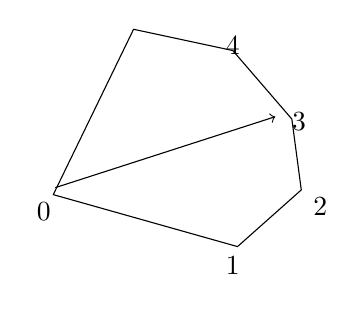
\begin{tikzpicture}[x=0.03cm,y=-0.03cm,line cap=round,line join=round]
\draw[thin] (0,70)--(34,0)--(76,9)--(101,38)--(105,68)--(78,92)--(0,70);
\draw[->] (1,67)--(94,37);
\node at (-4,77) {\handwritten{$0$}};
\node at (76,100) {\handwritten{$1$}};
\node at (113,75) {\handwritten{$2$}};
\node at (104,39) {\handwritten{$3$}};
\node at (76,7) {\handwritten{$4$}};
\end{tikzpicture}}

\figure{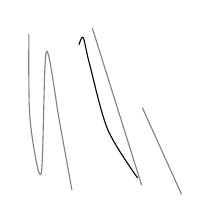
\begin{tikzpicture}[x=0.013cm,y=-0.013cm,line cap=round,line join=round]
\draw[gray,thin] plot[smooth] coordinates {(1,40) (2,122) (13,176) (18,57) (31,126) (43,192)};
\draw[thin] plot[smooth] coordinates {(50,50) (54,43) (60,68) (78,133) (107,180)};
\draw[gray,thin] (63,34)--(111,187);
\draw[gray,thin] (112,112)--(150,196);
\end{tikzpicture}}

\figure{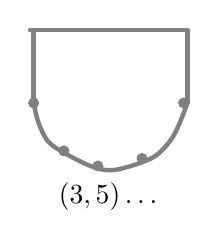
\begin{tikzpicture}[x=0.016cm,y=-0.016cm,line cap=round,line join=round]
\draw[gray,line width=1.6pt] (0,0)--(125,0)--(125,58);
\draw[gray,line width=1.6pt] (3,0)--(3,58);
\draw[gray,line width=1.6pt] plot[smooth] coordinates {(3,58) (7,74) (17,91) (48,108) (68,111) (98,101) (114,84) (125,58)};
\fill[gray] (3,58) circle [radius=2pt];
\fill[gray] (122,58) circle [radius=2pt];
\fill[gray] (27,96) circle [radius=2pt];
\fill[gray] (54,108) circle [radius=2pt];
\fill[gray] (89,102) circle [radius=2pt];
\node at (62,132) {\handwritten{$(3,5)\ldots$}};
\end{tikzpicture}}

\figure{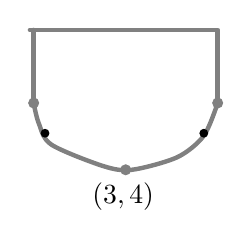
\begin{tikzpicture}[x=0.016cm,y=-0.016cm,line cap=round,line join=round]
\draw[gray,line width=1.6pt] (0,0)--(149,0)--(149,58);
\draw[gray,line width=1.6pt] (3,0)--(3,58);
\draw[gray,line width=1.6pt] plot[smooth] coordinates {(3,58) (7,74) (17,91) (58,108) (81,111) (117,101) (138,84) (149,58)};
\fill[gray] (3,58) circle [radius=2pt];
\fill[gray] (149,58) circle [radius=2pt];
\fill[gray] (76,111) circle [radius=2pt];
\fill[black] (12,82) circle [radius=1.6pt];
\fill[black] (138,82) circle [radius=1.6pt];
\node at (74,132) {\handwritten{$(3,4)$}};
\end{tikzpicture}}

\figure{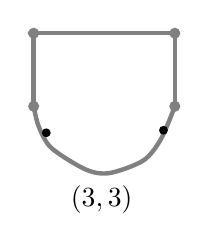
\begin{tikzpicture}[x=0.016cm,y=-0.016cm,line cap=round,line join=round]
\draw[gray,line width=1.6pt] (0,0)--(115,0)--(115,58);
\draw[gray,line width=1.6pt] (3,0)--(3,58);
\draw[gray,line width=1.6pt] plot[smooth] coordinates {(3,58) (7,74) (17,91) (44,108) (63,111) (90,101) (104,84) (115,58)};
\fill[gray] (3,0) circle [radius=2pt];
\fill[gray] (3,58) circle [radius=2pt];
\fill[gray] (115,0) circle [radius=2pt];
\fill[gray] (115,58) circle [radius=2pt];
\fill[black] (13,79) circle [radius=1.6pt];
\fill[black] (106,77) circle [radius=1.6pt];
\node at (57,132) {\handwritten{$(3,3)$}};
\end{tikzpicture}}

\handwritten{$2(\deleted{\unsure{n-2\nu}})$}

\figure{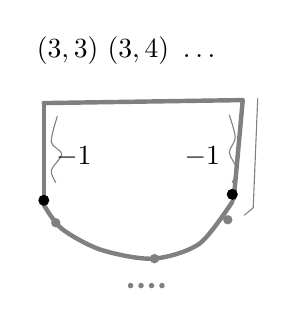
\begin{tikzpicture}[x=0.019cm,y=-0.019cm,line cap=round,line join=round]
\draw[gray,line width=1.6pt] (0,0)--(133,-2)--(127,64);
\draw[gray,line width=1.6pt] (0,0)--(0,68);
\draw[gray,line width=1.6pt] plot[smooth] coordinates {(0,68) (12,84) (38,98) (73,104) (104,94) (126,66)};
\draw[gray,thin] plot[smooth] coordinates {(9,9) (5,26) (12,34) (5,45) (8,53)};
\draw[gray,thin] plot[smooth] coordinates {(124,8) (128,23) (124,33) (129,44) (126,53)};
\draw[gray,thin] (143,-3)--(140,70)--(134,75);
\fill[black] (0,65) circle [radius=2pt];
\fill[black] (126,61) circle [radius=2pt];
\fill[gray] (8,80) circle [radius=1.7pt];
\fill[gray] (74,104) circle [radius=1.7pt];
\fill[gray] (123,78) circle [radius=1.7pt];
\fill[gray] (58,122) circle [radius=1pt];
\fill[gray] (65,122) circle [radius=1pt];
\fill[gray] (72,122) circle [radius=1pt];
\fill[gray] (79,122) circle [radius=1pt];
\node at (20,36) {\handwritten{$-1$}};
\node at (106,36) {\handwritten{$-1$}};
\node at (55,-35) {\handwritten{$(3,3)\ (3,4)\ \ldots$}};
\end{tikzpicture}}

\figure{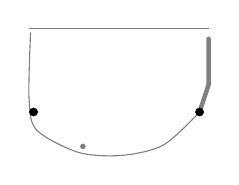
\begin{tikzpicture}[x=0.019cm,y=-0.019cm,line cap=round,line join=round]
\draw[gray,thin] (0,0)--(120,0);
\draw[gray,line width=1.6pt] (120,7)--(120,38)--(114,56);
\draw[gray,thin] plot[smooth] coordinates {(1,3) (0,47) (5,68) (33,83) (62,85) (90,78) (115,55)};
\fill[black] (3,56) circle [radius=1.6pt];
\fill[black] (114,56) circle [radius=1.6pt];
\fill[gray] (36,79) circle [radius=1pt];
\end{tikzpicture}}

\figure{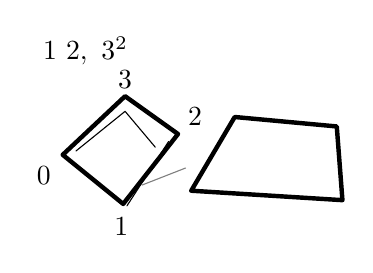
\begin{tikzpicture}[x=0.024cm,y=-0.024cm,line cap=round,line join=round]
\draw[line width=1.6pt] (0,31)--(33,0)--(61,20)--(32,57)--(0,31);
\draw[thin] (7,29)--(33,8)--(49,27);
\draw[thin] (56,24)--(34,58);
\draw[line width=1.6pt] (68,50)--(91,11)--(145,16)--(148,55)--(68,50);
\draw[gray,thin] (42,47)--(65,38);
\node at (-10,42) {\handwritten{$0$}};
\node at (31,69) {\handwritten{$1$}};
\node at (70,11) {\handwritten{$2$}};
\node at (33,-9) {\handwritten{$3$}};
\node at (12,-24) {\handwritten{$1\ 2,\ 3^{\unsure{2}}$}};
\end{tikzpicture}}

\figure{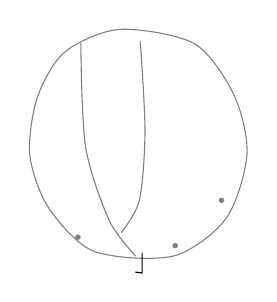
\begin{tikzpicture}[x=0.012cm,y=-0.012cm,line cap=round,line join=round]
\draw[gray,thin] plot[smooth cycle] coordinates {(40,33) (98,9) (177,24) (219,78) (233,141) (211,209) (155,249) (71,244) (23,198) (3,142) (11,81)};
\draw[gray,thin] plot[smooth] coordinates {(57,24) (62,133) (87,211) (115,249)};
\draw[gray,thin] plot[smooth] coordinates {(120,22) (125,117) (119,190) (100,224)};
\fill[gray] (54,229) circle [radius=1pt];
\fill[gray] (157,238) circle [radius=1pt];
\fill[gray] (206,190) circle [radius=1pt];
\draw[thin] (122,246)--(122,267)--(115,266);
\end{tikzpicture}}

\figure{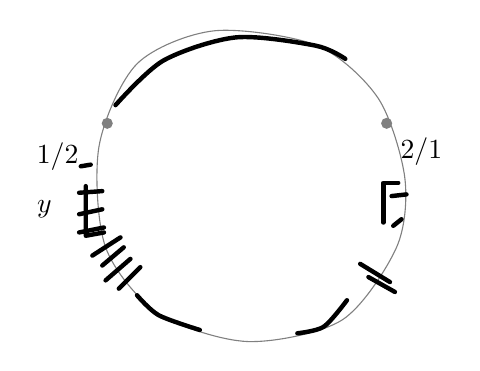
\begin{tikzpicture}[x=0.021cm,y=-0.021cm,line cap=round,line join=round]
\draw[gray,thin] plot[smooth cycle] coordinates {(12,71) (35,21) (82,1) (144,10) (181,42) (197,90) (192,132) (159,176) (102,189) (48,172) (16,132)};
\draw[line width=1.6pt] plot[smooth] coordinates {(22,46) (51,19) (95,5) (143,10) (161,18)};
\draw[line width=1.6pt] (1,83)--(7,82);
\draw[line width=1.6pt] (4,95)--(4,125)--(15,123);
\draw[line width=1.6pt] (0,99)--(14,98);
\draw[line width=1.6pt] (0,112)--(14,109);
\draw[line width=1.6pt] (0,123)--(15,120);
\draw[line width=1.6pt] (8,137)--(25,126);
\draw[line width=1.6pt] (14,143)--(27,132);
\draw[line width=1.6pt] (16,152)--(31,139);
\draw[line width=1.6pt] (24,157)--(37,144);
\draw[line width=1.6pt] plot[smooth] coordinates {(35,161) (48,173) (73,182)};
\draw[line width=1.6pt] plot[smooth] coordinates {(132,184) (148,180) (162,164)};
\draw[line width=1.6pt] (175,150)--(191,159);
\draw[line width=1.6pt] (170,142)--(188,153);
\draw[line width=1.6pt] (184,117)--(184,93)--(193,93);
\draw[line width=1.6pt] (190,119)--(195,115);
\draw[line width=1.6pt] (189,101)--(198,100);
\fill[gray] (17,57) circle [radius=2pt];
\fill[gray] (186,57) circle [radius=2pt];
\node at (-13,77) {\handwritten{$\unsure{1/2}$}};
\node at (207,74) {\handwritten{$\unsure{2/1}$}};
\node at (-21,109) {\handwritten{$\unsure{y}$}};
\end{tikzpicture}}

\figure{\begin{tikzpicture}[x=0.018cm,y=-0.018cm,line cap=round,line join=round]
\draw[gray,thin] plot[smooth] coordinates {(45,0) (50,52) (29,117) (1,188) (36,172) (76,144) (72,158)};
\draw[gray,thin] (6,282)--(0,299);
\end{tikzpicture}}

\figure{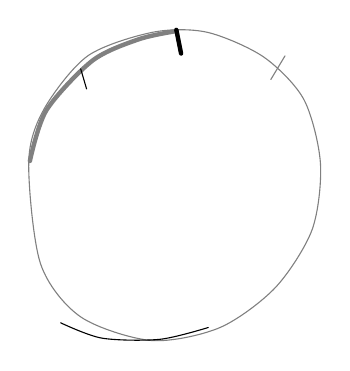
\begin{tikzpicture}[x=0.015cm,y=-0.015cm,line cap=round,line join=round]
\draw[gray,thin] plot[smooth cycle] coordinates {(5,118) (18,73) (55,28) (110,8) (156,8) (204,29) (238,65) (252,119) (245,175) (214,224) (167,258) (109,269) (49,249) (15,204)};
\draw[gray,line width=1.6pt] plot[smooth] coordinates {(6,117) (20,74) (59,32) (98,14) (130,7)};
\draw[line width=1.6pt] (130,6)--(134,26);
\draw[thin] (49,39)--(54,56);
\draw[gray,thin] (210,48)--(222,28);
\draw[thin] plot[smooth] coordinates {(32,254) (67,267) (116,268) (157,258)};
\end{tikzpicture}}

\figure{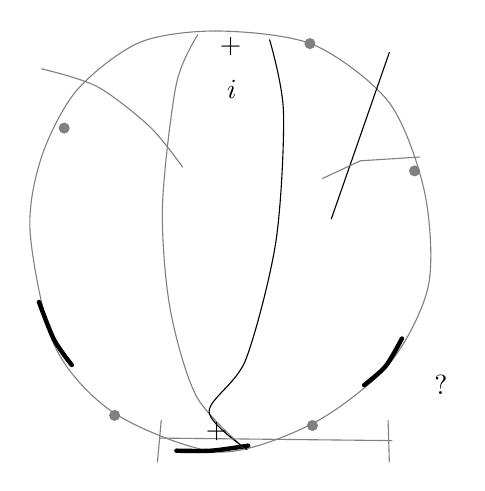
\begin{tikzpicture}[x=0.016cm,y=-0.016cm,line cap=round,line join=round]
\draw[gray,thin] plot[smooth cycle] coordinates {(1,160) (10,100) (38,47) (88,9) (151,0) (226,11) (286,57) (314,128) (317,202) (286,264) (226,311) (151,334) (69,304) (21,251)};
\draw[line width=1.6pt] plot[smooth] coordinates {(8,215) (20,245) (34,265)};
\draw[line width=1.6pt] plot[smooth] coordinates {(266,281) (283,266) (296,244)};
\draw[line width=1.6pt] plot[smooth] coordinates {(117,333) (145,333) (174,329)};
\draw[gray,thin] plot[smooth] coordinates {(134,3) (117,42) (106,139) (112,220) (133,290) (172,332)};
\draw[thin] plot[smooth] coordinates {(191,7) (202,64) (196,167) (172,261) (143,302) (173,332)};
\draw[gray,thin] (104,323)--(288,325);
\draw[gray,thin] (105,309)--(102,342);
\draw[gray,thin] (285,309)--(286,342);
\draw[gray,thin] plot[smooth] coordinates {(10,30) (54,44) (96,76) (122,108)};
\draw[thin] (240,149)--(286,17);
\draw[gray,thin] (233,117)--(263,103)--(310,100);
\fill[gray] (28,77) circle [radius=2pt];
\fill[gray] (223,10) circle [radius=2pt];
\fill[gray] (306,111) circle [radius=2pt];
\fill[gray] (225,313) circle [radius=2pt];
\fill[gray] (68,305) circle [radius=2pt];
\node at (160,12) {\handwritten{$+$}};
\node at (161,46) {\handwritten{$\unsure{i}$}};
\node at (149,318) {\handwritten{$\unsure{+}$}};
\node at (327,281) {\handwritten{$\unsure{?}$}};
\end{tikzpicture}}

\figure{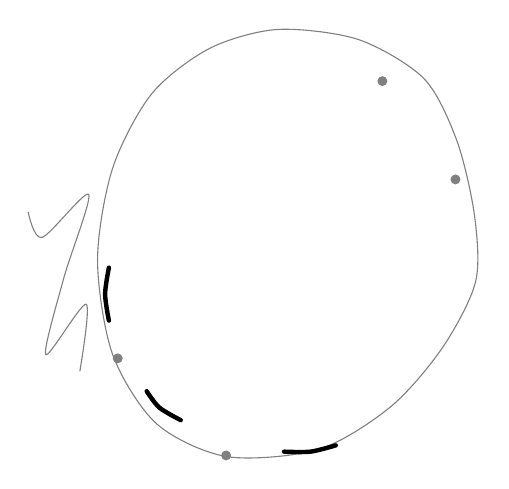
\begin{tikzpicture}[x=0.016cm,y=-0.016cm,line cap=round,line join=round]
\draw[gray,thin] plot[smooth cycle] coordinates {(1,183) (13,110) (44,51) (90,15) (144,0) (208,8) (260,39) (286,88) (300,147) (301,200) (275,252) (234,299) (177,333) (104,339) (48,313) (13,258)};
\draw[line width=1.6pt] plot[smooth] coordinates {(10,189) (7,210) (10,231)};
\draw[line width=1.6pt] plot[smooth] coordinates {(40,287) (50,300) (67,310)};
\draw[line width=1.6pt] plot[smooth] coordinates {(149,335) (170,335) (190,330)};
\draw[gray,thin] plot[smooth] coordinates {(-54,145) (-43,165) (-6,131) (-26,198) (-40,258) (-8,218) (-13,271)};
\fill[gray] (227,41) circle [radius=1.8pt];
\fill[gray] (285,119) circle [radius=1.8pt];
\fill[gray] (17,261) circle [radius=1.8pt];
\fill[gray] (103,338) circle [radius=1.8pt];
\end{tikzpicture}}
